\chapter{Arhitektura i dizajn sustava}
		
		Arhitektura aplikacije "Čuvari pasa" može se podijeliti na web poslužitelj, web aplikaciju i bazu podataka.
		\\
		\newline
		\textbf{Web poslužitelj} je zapravo funkcionalnost web aplikacije. On komunicira s klijentom preko web preglednika. Primarna uloga mu je "nabavljanje" HTTP zahtjeva i slanje HTTP odgovora. Ovisno o zahtjevu, web poslužitelj komunicira i s bazom podataka u kojoj se nalaze potrebni podaci. 
		\newline
		\textbf{Web preglednik} je softver koji služi kao sučelje između poslužitelja i klijenta i prikaz web dokumenta klijentu. Njegova primarna uloga je slanje HTTP zahtjeva i primanje HTTP odgovora. Web preglednici prevode kod koji dobivaju u HTTP odgovoru te ga zatim prikazuju.
		\newline
		\textbf{Baza podataka} (podatkovni sloj) koristi se za sigurno spremanje podataka. Povezana je s web aplikacijom koja joj šalje upite za potrebnim podacima. Baza podataka je dalje opisana u poglavlju 4.1 Baza podataka.
		\newline
		\textbf{Web aplikacija} podijeljena je na back-end i front-end. 
		\newline
		\textbf{Back-end} je dio sustava u kojem se zapravo obrađuju zahtjevi i vrše daljnje akcije. Njegova organizacija na kontrolere, servise i repozitorije pomaže u "razdvajanju zabrinutosti".
		Kontroleri upravljaju REST sučeljima prema poslovnoj logici koja je implementirana u servisima. Repozitoriji su zaslužni za spremanje i dohvaćanje nekog skupa podataka.
		Back-end također sadrži DTO-e (Data Transfer Object) i Domain modele. DTO-i se koriste za razmjenu podataka između procesa ili slojeva, a Domain modeli služe za razmjenu podataka s bazom podataka.
		\newline
		\textbf{Front-end} je prezentacijski dio aplikacije odnosno kako korisnik vidi aplikaciju u web pregledniku.
		\newline
		Front-end smo odlučili raditi u programskom jeziku JavaScript koristeći radni okvir React, a back-end u programskom jeziku Java s radnim okvirom Spring Boot. Razvojna okruženja u kojima radimo su Visual Studio Code i IntelliJ.
		
		\begin{figure}[htb]
			\centering
			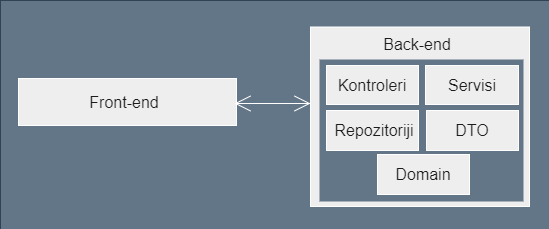
\includegraphics[width=14cm]{slike/Arhitektura}
			\caption{Dijagram arhitekture web aplikacije} 
			\label{fig:arhitektura-dijagram}
		\end{figure}
		
		\eject
				
		\section{Baza podataka}
			
			Sustav koristi relacijsku bazu podataka koja će biti implementirana u PostgreSQL-u. Relacijsku bazu podataka koristimo radi lakšeg oblikovanja sustava kao stvarnog svijeta, a PostgreSQL jer smo najbolje upoznati s njim. U njemu se entiteti modeliraju kao tablice koje imaju vlastito ime i skup atributa.\\
			Baza podataka nam je potrebna zbog njezine sigurnosti podataka, ali i brzog dohvata, pohrane i izmijene podataka koje sustav koristi za daljnje akcije.
			Baza podataka ovog sustava koristiti će sjedeće entitete:
			\begin{packed_item}
				\item role
				\item appuser
				\item breed
				\item dog
				\item request\_dog
				\item request\_guardian
				\item request\_guardians\_dog
				\item activity
				\item request\_activity
				\item agreed\_request
				
			\end{packed_item}
			
		
			\subsection{Opis tablica}
			
			\textbf{role} je entitet koji sadrži sve važne informacije o ulogama korisnika u aplikaciji. Sastoji se od atributa: role\_id, name. Povezan je vezom \textit{One-To-Many} s tablicom appuser preko vlastitog atributa role\_id. 
			\begin{longtblr}[
				label=none,
				entry=none
				]{
					width = \textwidth,
					colspec={|X[6,l]|X[6, l]|X[20, l]|}, 
					rowhead = 1,
				} %definicija širine tablice, širine stupaca, poravnanje i broja redaka naslova tablice
				\hline \multicolumn{3}{|c|}{\textbf{role}}	 \\ \hline[3pt]
				\SetCell{LightGreen}role\_id	& INT &  Jedinstveni identifikator uloge korisnika 	\\ \hline
				name & VARCHAR &  Naziv uloge u sustavu \\ \hline
			\end{longtblr}
			
			
			\textbf{appuser} je entitet koji sadrži sve važne informacije o korisniku aplikacije. Sastoji se od atributa: user\_id, role\_id, username, first\_name, last\_name, password, rating\_sum, rating\_count, email, has\_dog, has\_experience, blocked. Povezan je vezom \textit{Many-To-One} s tablicom role preko atributa role\_id tablice role. S tablicom dog je povezan vezom \textit{One-To-Many} preko vlastitog atributa user\_id. Isto vrijedi za tablice request\_dog i request\_guardian. S tablicom agreed\_request ima dvije veze, a to su \textit{One-To-Many} i \textit{One-To-One} preko vlastitog atributa user\_id.
			\begin{longtblr}[
				label=none,
				entry=none
				]{
					width = \textwidth,
					colspec={|X[6,l]|X[6, l]|X[20, l]|}, 
					rowhead = 1,
				} %definicija širine tablice, širine stupaca, poravnanje i broja redaka naslova tablice
				\hline \multicolumn{3}{|c|}{\textbf{appuser}}	 \\ \hline[3pt]
				\SetCell{LightGreen}user\_id & INT	&  	Jedinstveni identifikator korisnika\\ \hline
				\SetCell{LightBlue}role\_id	& INT &  Jedinstven identifikator uloge korisnika (role.role\_id) \\ \hline
				username & VARCHAR &  Korisničko ime u sustavu \\ \hline 
				first\_name & VARCHAR	&  	Ime korisnika	\\ \hline
				last\_name & VARCHAR	&  	Prezime korisnika	\\ \hline
				password & VARCHAR	&  	Hash lozinke korisnika	\\ \hline 
				rating\_sum & INT	&  	Zbroj svih ocjena	\\ \hline 
				rating\_count & INT	&  	Broj svih ocjenjivanja	\\ \hline 
				email & VARCHAR	&  	Email korisnika	\\ \hline 
				has\_dog & BOOLEAN	&  	Ima li korisnik psa	\\ \hline 
				has\_experience & BOOLEAN	&  	Ima li korisnik iskustvo	\\ \hline
				blocked & BOOLEAN	&  	Je li korisnik blokiran	\\ \hline  
			\end{longtblr}
			
			
			\textbf{breed} je entitet koji razlikuje sve pasmine u sustavu. Sastoji se od atributa: breed\_id, name. Povezan je vezom \textit{One-To-Many} s tablicom dog preko vlastitog atributa breed\_id. Isto vrijedi i za tablicu request\_dog. 
			\begin{longtblr}[
				label=none,
				entry=none
				]{
					width = \textwidth,
					colspec={|X[6,l]|X[6, l]|X[20, l]|}, 
					rowhead = 1,
				} %definicija širine tablice, širine stupaca, poravnanje i broja redaka naslova tablice
				\hline \multicolumn{3}{|c|}{\textbf{breed}}	 \\ \hline[3pt]
				\SetCell{LightGreen}breed\_id & INT	&  	Jedinstveni identifikator pasmine\\ \hline
				name	& VARCHAR &  Naziv pasmine	\\ \hline 
			\end{longtblr}
		
		
			\textbf{dog} je entitet koji sadrži sve važne informacije o psima vlasnika. Sastoji se od atributa: dog\_id, name, rating\_sum, rating\_count, user\_id, breed\_id, date\_of\_birth, photo. Povezan je vezom \textit{Many-To-One} s tablicom appuser preko atributa user\_id tablice appuser i istom takvom vezom s tablicom breed preko atributa breed\_id tablice breed. Vezom \textit{One-To-One} povezan je s tablicom request\_guardians\_dog preko vlastitog atributa dog\_id. 
			\begin{longtblr}[
				label=none,
				entry=none
				]{
					width = \textwidth,
					colspec={|X[6,l]|X[6, l]|X[20, l]|}, 
					rowhead = 1,
				} %definicija širine tablice, širine stupaca, poravnanje i broja redaka naslova tablice
				\hline \multicolumn{3}{|c|}{\textbf{dog}}	 \\ \hline[3pt]
				\SetCell{LightGreen}dog\_id & INT	&  	Jedinstveni identifikator psa\\ \hline
				name	& VARCHAR &  Ime psa	\\ \hline 
				rating\_sum	& INT &  Zbroj svih ocjena	\\ \hline
				rating\_count	& INT &  Broj svih ocjenjivanja	\\ \hline
				\SetCell{LightBlue}user\_id	& INT &  Jedinstveni identifikator vlasnika psa (appuser.user\_id)	\\ \hline
				\SetCell{LightBlue}breed\_id	& INT &  Jedinstveni identifikator pasmine (breed.breed\_id)	\\ \hline
				date\_of\_birth	& DATE &  Datum rođenja psa	\\ \hline 
				photo	& BYTEA &  Slika psa	\\ \hline	
			\end{longtblr}


			\textbf{request\_dog} je entitet koji sadrži sve važne informacije o oglasima koje čuvari pasa objavljuju. Sastoji se od atributa: request\_dog\_id, dog\_age, dog\_time\_begin, dog\_time\_end, is\_flexible, location, number\_of\_dogs, is\_published, is\_reviewed, bre-ed\_id, user\_id, location\_name. Povezan je vezom \textit{Many-To-One} s tablicom breed preko atributa breed\_id tablice breed i istom takvom vezom s tablicom appuser preko atributa user\_id tablice appuser. Vezom \textit{One-To-One} je povezan s tablicom agre-ed\_request preko vlastitog atributa request\_dog\_id. 
			\begin{longtblr}[
				label=none,
				entry=none
				]{
					width = \textwidth,
					colspec={|X[7,l]|X[6, l]|X[20, l]|}, 
					rowhead = 1,
				} %definicija širine tablice, širine stupaca, poravnanje i broja redaka naslova tablice
				\hline \multicolumn{3}{|c|}{\textbf{request\_dog}}	 \\ \hline[3pt]
				\SetCell{LightGreen}request\_dog\_id & INT	&  	Jedinstveni identifikator oglasa za čuvanje pasa\\ \hline
				dog\_age	& INT &  Preferirana dob pasa	\\ \hline 
				dog\_time\_begin	& TIMESTAMP  &  Početak čuvanja pasa	\\ \hline 
				dog\_time\_end	& TIMESTAMP  &  Završetak čuvanja pasa	\\ \hline
				is\_flexible	& BOOLEAN &  Je li vrijeme čuvanja fleksibilno	\\ \hline
				location	& VARCHAR &  Koordinate lokacije čuvanja pasa	\\ \hline
				number\_of\_dogs	& INT &  Broj pasa	\\ \hline
				is\_pusblished	& BOOLEAN &  Je li oglas objavljen	\\ \hline
				is\_reviewed	& BOOLEAN &  Je li oglas pregledan od strane administratora	\\ \hline
				\SetCell{LightBlue}breed\_id	& INT &  Jedinstveni identifikator pasmine (breed.breed\_id)	\\ \hline
				\SetCell{LightBlue}user\_id	& INT &  Jedinstveni identifikator čuvara pasa (appuser.user\_id)	\\ \hline
				location\_name	& VARCHAR &  Naziv lokacije čuvanja pasa	\\ \hline
			\end{longtblr}
		
		
			\textbf{request\_guardian} je entitet koji sadrži sve važne informacije o zahtjevima koje vlasnici pasa objavljuju. Sastoji se od atributa: request\_guardian\_id, location, number\_of\_dogs, guard\_time\_begin, guard\_time\_end, is\_published, is\_reviewed, user\_id, has\_experience, has\_dog, location\_name. Povezan je vezom \textit{Many-To-One} s tablicom appuser preko atributa user\_id tablice appuser. S tablicama request\_guar-dians\_dog i request\_activity povezan je vezom \textit{One-To-Many} preko vlastitog atributa request\_guardian\_id. Vezom \textit{One-To-One} je povezan s tablicom agreed\_request preko vlastitog atributa request\_guardian\_id.
			\begin{longtblr}[
				label=none,
				entry=none
				]{
					width = \textwidth,
					colspec={|X[10,l]|X[6, l]|X[20, l]|}, 
					rowhead = 1,
				} %definicija širine tablice, širine stupaca, poravnanje i broja redaka naslova tablice
				\hline \multicolumn{3}{|c|}{\textbf{request\_guardian}}	 \\ \hline[3pt]
				\SetCell{LightGreen}request\_guardian\_id & INT	&  	Jedinstveni identifikator zahtjeva za čuvanje pasa\\ \hline
				location	& VARCHAR &  Koordinate lokacije čuvanja pasa	\\ \hline 
				number\_of\_dogs	& INT &  Broj pasa	\\ \hline
				guard\_time\_begin	& TIMESTAMP  &  Početak čuvanja pasa	\\ \hline 
				guard\_time\_end	& TIMESTAMP  &  Završetak čuvanja pasa	\\ \hline
				is\_published	& BOOLEAN &  Je li zahtjev objavljen	\\ \hline
				is\_reviewed	& BOOLEAN &  Je li zahtjev pregledan od strane administratora	\\ \hline
				\SetCell{LightBlue}user\_id	& INT &  Jedinstveni identifikator vlasnika pasa (appuser.user\_id)	\\ \hline
				has\_experience	& BOOLEAN &  Želi li vlasnik da čuvar ima iskustvo	\\ \hline
				has\_dog	& BOOLEAN &  Želi li vlasnik da čuvar ima vlastitog psa	\\ \hline
				location\_name	& VARCHAR &  Naziv lokacije čuvanja pasa	\\ \hline				
			\end{longtblr}
		
		
			\textbf{request\_guardians\_dog} je entitet koji sadrži sve važne informacije o psima koji su povezani s pojedinim zahtjevima za čuvanje koje je objavio vlasnik pasa. Potreban je kako bi se unutar jednog zahtjeva za čuvanje moglo nalaziti više pasa koje je potrebno istovremeno čuvati. Sastoji se od atributa: request\_guardians\_dog\_id, request\_guardian\_id, dog\_id. Povezan je vezom \textit{One-To-One} s tablicom dog preko atributa dog\_id tablice dog. S tablicom request\_guardian povezan je vezom \textit{Many-To-One} preko atributa request\_guardian\_id tablice request\_guardian. 
			\begin{longtblr}[
				label=none,
				entry=none
				]{
					width = \textwidth,
					colspec={|X[13,l]|X[6, l]|X[20, l]|}, 
					rowhead = 1,
				} %definicija širine tablice, širine stupaca, poravnanje i broja redaka naslova tablice
				\hline \multicolumn{3}{|c|}{\textbf{request\_guardians\_dog}}	 \\ \hline[3pt]
				\SetCell{LightGreen}request\_guardians\_dog\_id & INT	&  	Jedinstveni identifikator psa povezanog sa zahtjevom za čuvanje pasa\\ \hline
				\SetCell{LightBlue}request\_guardian\_id	& INT &  Jedinstveni identifikator zahtjeva za čuvanje pasa (request\_guardian. request\_guardian\_id)	\\ \hline
				\SetCell{LightBlue}dog\_id	& INT &  Jedinstveni identifikator psa (dog.dog\_id)	\\ \hline
			\end{longtblr}			
		
		
			\textbf{activity} je entitet koji sadrži sve važne informacije o aktivnosti koje bi pas i čuvar trebali raditi. Sastoji se od atributa: activity\_id, activity\_name. Povezan je vezom \textit{One-To-Many} s tablicom request\_activity preko vlastitog atributa activity\_id.
			\begin{longtblr}[
				label=none,
				entry=none
				]{
					width = \textwidth,
					colspec={|X[6,l]|X[6, l]|X[20, l]|}, 
					rowhead = 1,
				} %definicija širine tablice, širine stupaca, poravnanje i broja redaka naslova tablice
				\hline \multicolumn{3}{|c|}{\textbf{activity}}	 \\ \hline[3pt]
				\SetCell{LightGreen}activity\_id & INT	&  Jedinstveni identifikator aktivnosti \\ \hline
				activity\_name	& VARCHAR &  Naziv aktivnosti	\\ \hline
			\end{longtblr}			
		
		
			\textbf{request\_activity} je entitet koji sadrži sve važne informacije o aktivnostima koje su povezane s pojedinim zahtjevima za čuvanje koje su objavili vlasnici pasa. Potreban je kako bi se unutar jednog zahtjeva za čuvanje moglo nalaziti više aktivnosti koje je potrebno raditi sa psima tijekom čuvanja. Sastoji se od atributa: request\_activity\_id, activity\_id, feeding\_quantitiy, request\_guardian\_id. Povezan je vezom \textit{Many-To-One} s tablicom activity preko atributa activity\_id tablice activity i istom takvom vezom s tablicom request\_guardian preko atributa request\_guardian\_id tablice request\_guardian.  
			\begin{longtblr}[
				label=none,
				entry=none
				]{
					width = \textwidth,
					colspec={|X[10,l]|X[6, l]|X[20, l]|}, 
					rowhead = 1,
				} %definicija širine tablice, širine stupaca, poravnanje i broja redaka naslova tablice
				\hline \multicolumn{3}{|c|}{\textbf{request\_activity}}	 \\ \hline[3pt]
				\SetCell{LightGreen}request\_activity\_id & INT	&  Jedinstveni identifikator aktivnosti povezane sa zahtjevom za čuvanje pasa \\ \hline
				\SetCell{LightBlue}activity\_id	& INT &  Jedinstveni identifikator aktivnosti (activity.activitity\_id)	\\ \hline
				feeding\_quantity	& INT &  Količina hrane ukoliko je odabrana aktivnost koja uključuje hranu	\\ \hline
				\SetCell{LightBlue}request\_guardian\_id	& INT &  Jedinstveni identifikator zahtjeva za čuvanje pasa (request\_guardian.request\_guardian\_id) \\ \hline
			\end{longtblr}	
	
	
			\textbf{agreed\_request} je entitet koji sadrži sve važne informacije o dogovorenim/ nedogovorenim zahtjevima i oglasima za čuvanje od strane vlasnika i čuvara. Sastoji se od atributa: agreed\_request\_id, is\_agreed, agreed\_time\_begin, agreed\_time\_end, request\_guardian\_id, request\_dog\_id, initiator\_user\_id, user\_id, initiator\_rated, us-er\_rated. Povezan je vezom \textit{One-To-One} s tablicom request\_guardian preko atributa request\_guardian\_id tablice request\_guardian, istom takvom vezom s tablicom request\_dog preko atributa request\_dog\_id tablice request\_dog te istom takvom vezom s tablicom appuser preko atributa user\_id tablice appuser. S tablicom appuser još je povezan vezom \textit{Many-To-One} preko atributa initiator\_user\_id koji zapravo predstavlja atribut user\_id tablice appuser.
			\begin{longtblr}[
				label=none,
				entry=none
				]{
					width = \textwidth,
					colspec={|X[10,l]|X[6, l]|X[20, l]|}, 
					rowhead = 1,
				} %definicija širine tablice, širine stupaca, poravnanje i broja redaka naslova tablice
				\hline \multicolumn{3}{|c|}{\textbf{agreed\_request}}	 \\ \hline[3pt]
				\SetCell{LightGreen}agreed\_request\_id & INT	&  Jedinstveni identifikator dogovorenih/ nedogovorenih zahtjeva i oglasa za čuvanje \\ \hline
				is\_agreed	& BOOLEAN &  Je li postignut dogovor	\\ \hline
				agreed\_time\_begin	& TIMESTAMP &  Dogovoren početak čuvanja \\ \hline
				agreed\_time\_end	& TIMESTAMP &  Dogovoren kraj čuvanja	\\ \hline
				\SetCell{LightBlue}request\_guardian\_id	& INT &  Jedinstveni identifikator zahtjeva za čuvanje pasa (request\_guardian.request\_guardian\_id) \\ \hline
				\SetCell{LightBlue}request\_dog\_id	& INT &  Jedinstveni identifikator oglasa za čuvanje pasa (request\_dog.request\_dog\_id)\\ \hline
				\SetCell{LightBlue}initiator\_user\_id	& INT &  Jedinstveni identifikator korisnika koji je započeo interakciju (appuser.user\_id) \\ \hline
				\SetCell{LightBlue}user\_id	& INT &  Jedinstveni identifikator korisnika s kojim je započeta interakcija (appuser.user\_id) \\ \hline
				initiator\_rated	& BOOLEAN &  Je li korisnik koji je započeo interakciju ocijenio iskustvo \\ \hline
				user\_rated	& BOOLEAN &  Je li korisnik s kojim je započeta interakcija ocijenio iskustvo \\ \hline
			\end{longtblr}	
			
			\eject
			\subsection{Dijagram baze podataka}
			
			\begin{figure}[htb]
				\centering
				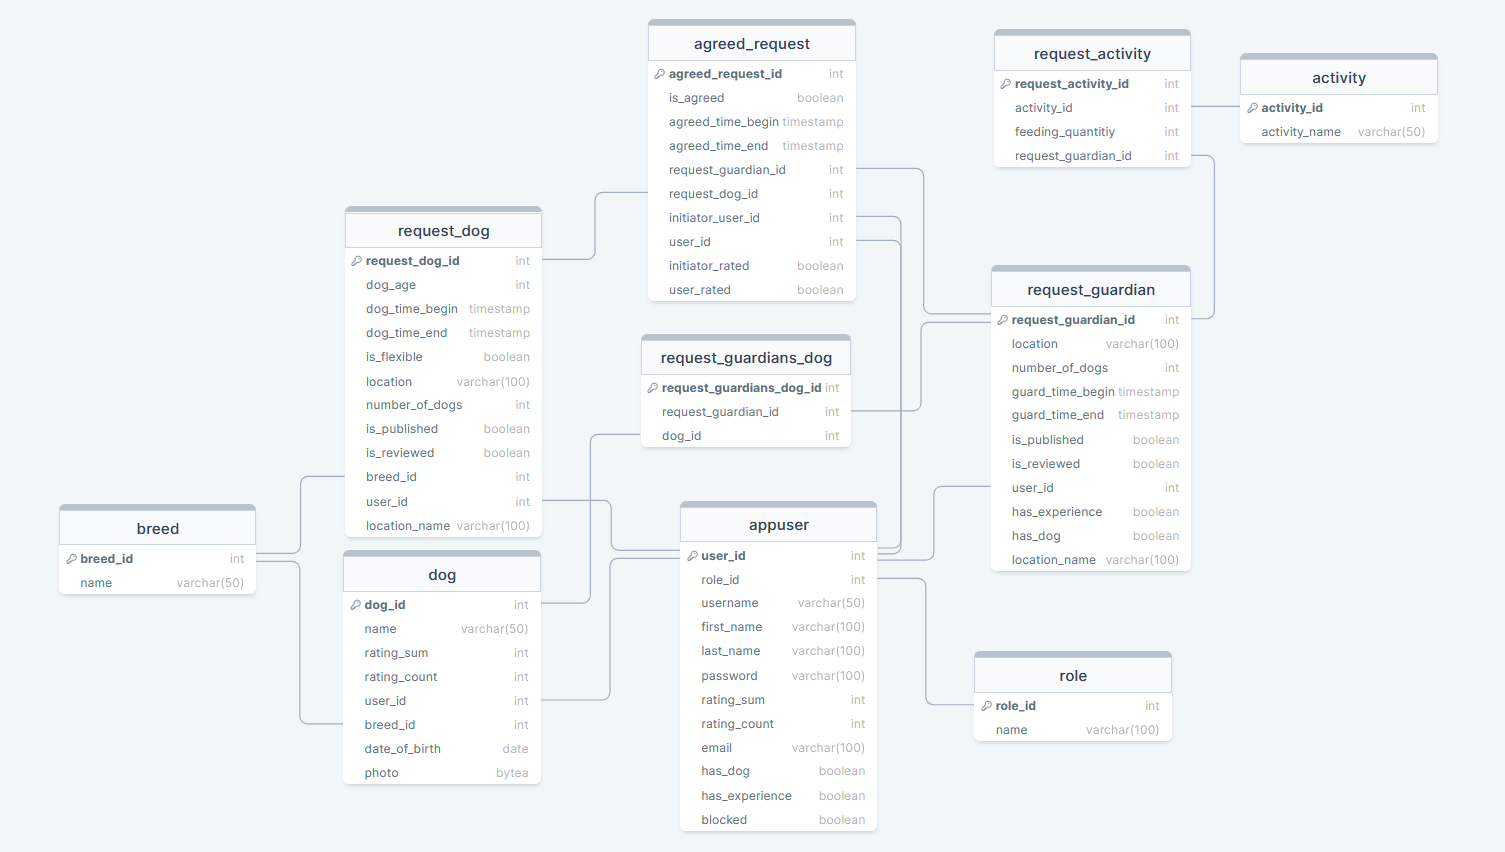
\includegraphics[width=15cm]{slike/drawsql REL}
				\caption{Relacijski dijagram baze podataka} 
				\label{fig:RelDiagram}
			\end{figure}
			
			\eject
			
			
		\section{Dijagram razreda}
		
			Na slikama 4.3, 4.4 i 4.5 prikazani su razredi koji pripadaju backend dijelu s arhitekturom podijeljenom na kontrolere, repozitorije i servise te uključuju Domain i DTO (Data Transfer Object) modele.\\
			Na slici 4.3 prikazani su razredi koji nasljeđuju Controller razred. Metode implementirane u tim razredima manipuliraju s DTO-ima, a oni su dohvaćeni pomoću metoda implementiranih u Domain razredima.
			
			\begin{figure}[htb]
				\centering
				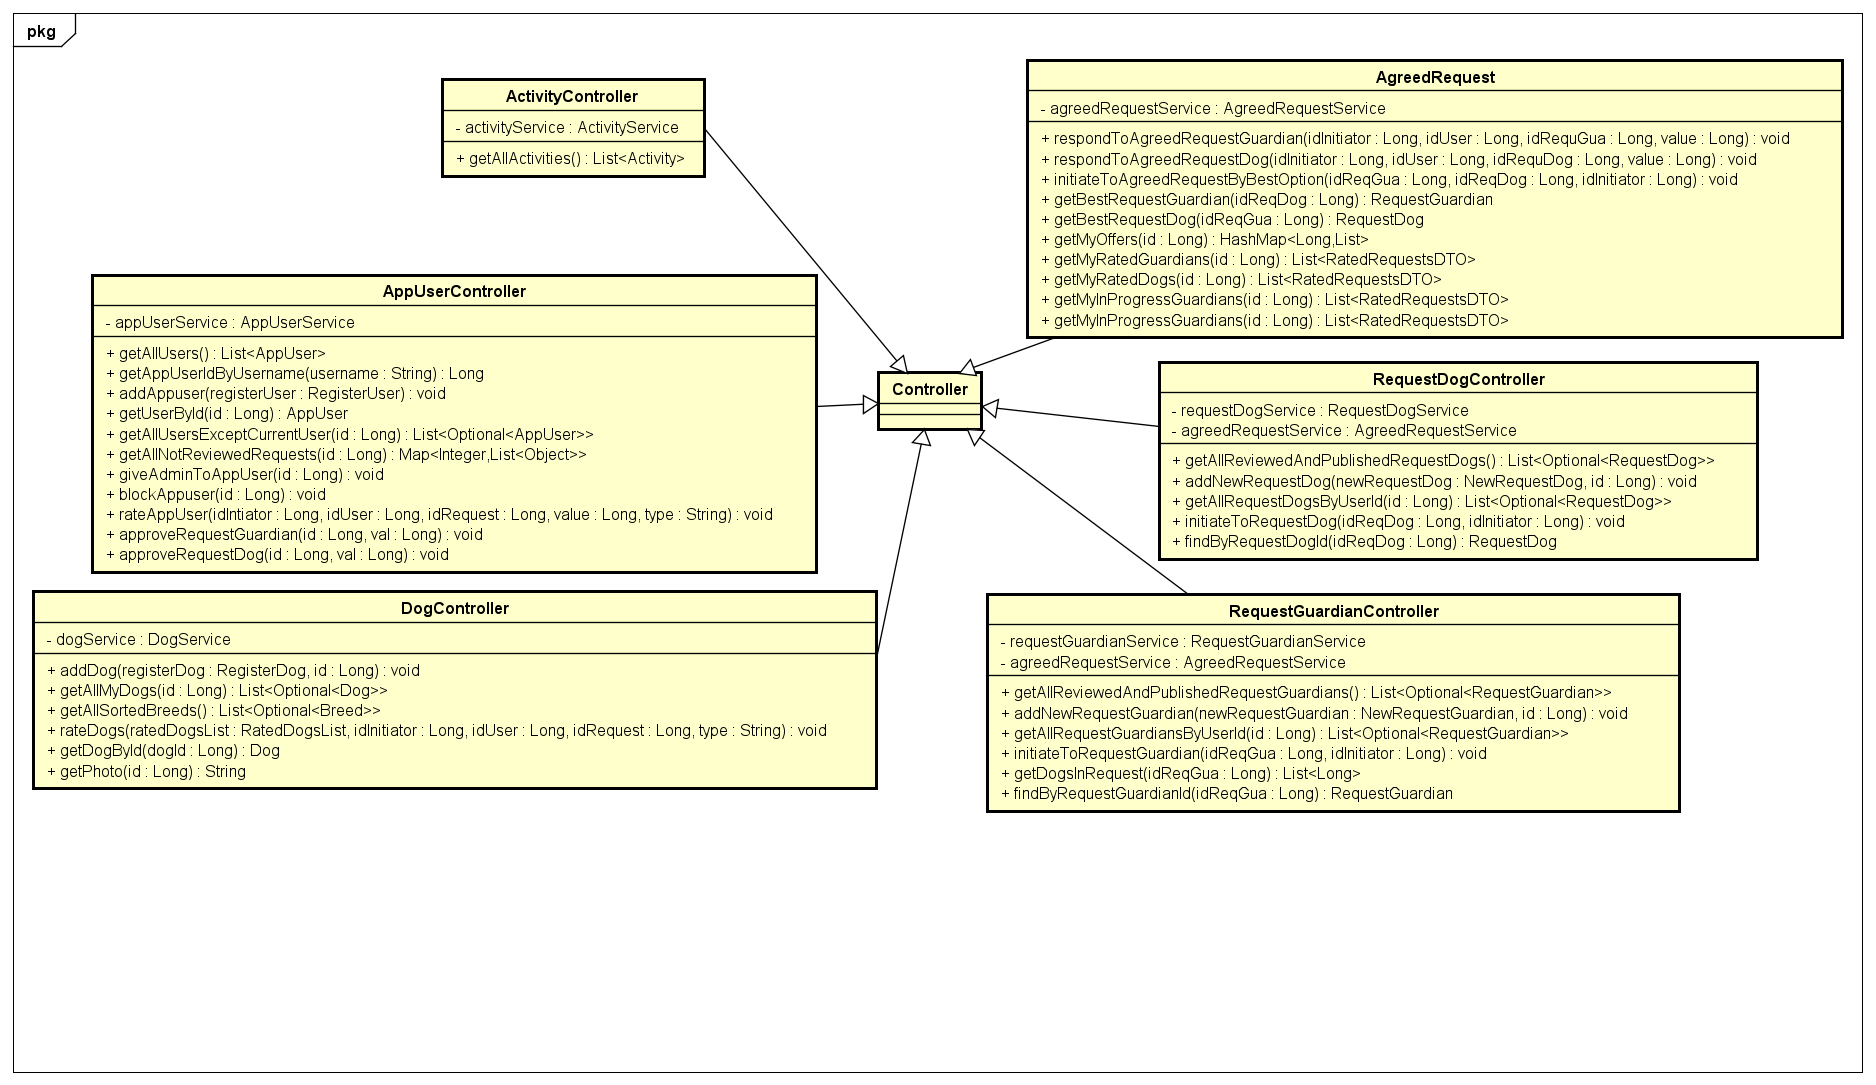
\includegraphics[width=15cm]{slike/Dijagram razreda - Controllers}
				\caption{Dijagram razreda - dio Controllers} 
				\label{fig:Class-Diagram}
			\end{figure}
		
		
			Data Transfer Objects služe za razmjenu podataka između procesa ili slojeva.
			RegisterUser i ReqisterDog služe za stvaranje novog objekta User, odnosno Dog.
			NewRequestDog i NewRequestGuardian služe za stvaranje novog objekta RequestDog, odnosno RequestGuardian.
			RatedDogsList služi za primanje podataka o ocijenjenim psima.
			RequestGuardianDTO, RequestBothDTO, RatedRequestsDTO služe kao pomoćni objekti za čitanje tih objekata iz baze podataka.
			\eject
			
			\begin{figure}[htb]
				\centering
				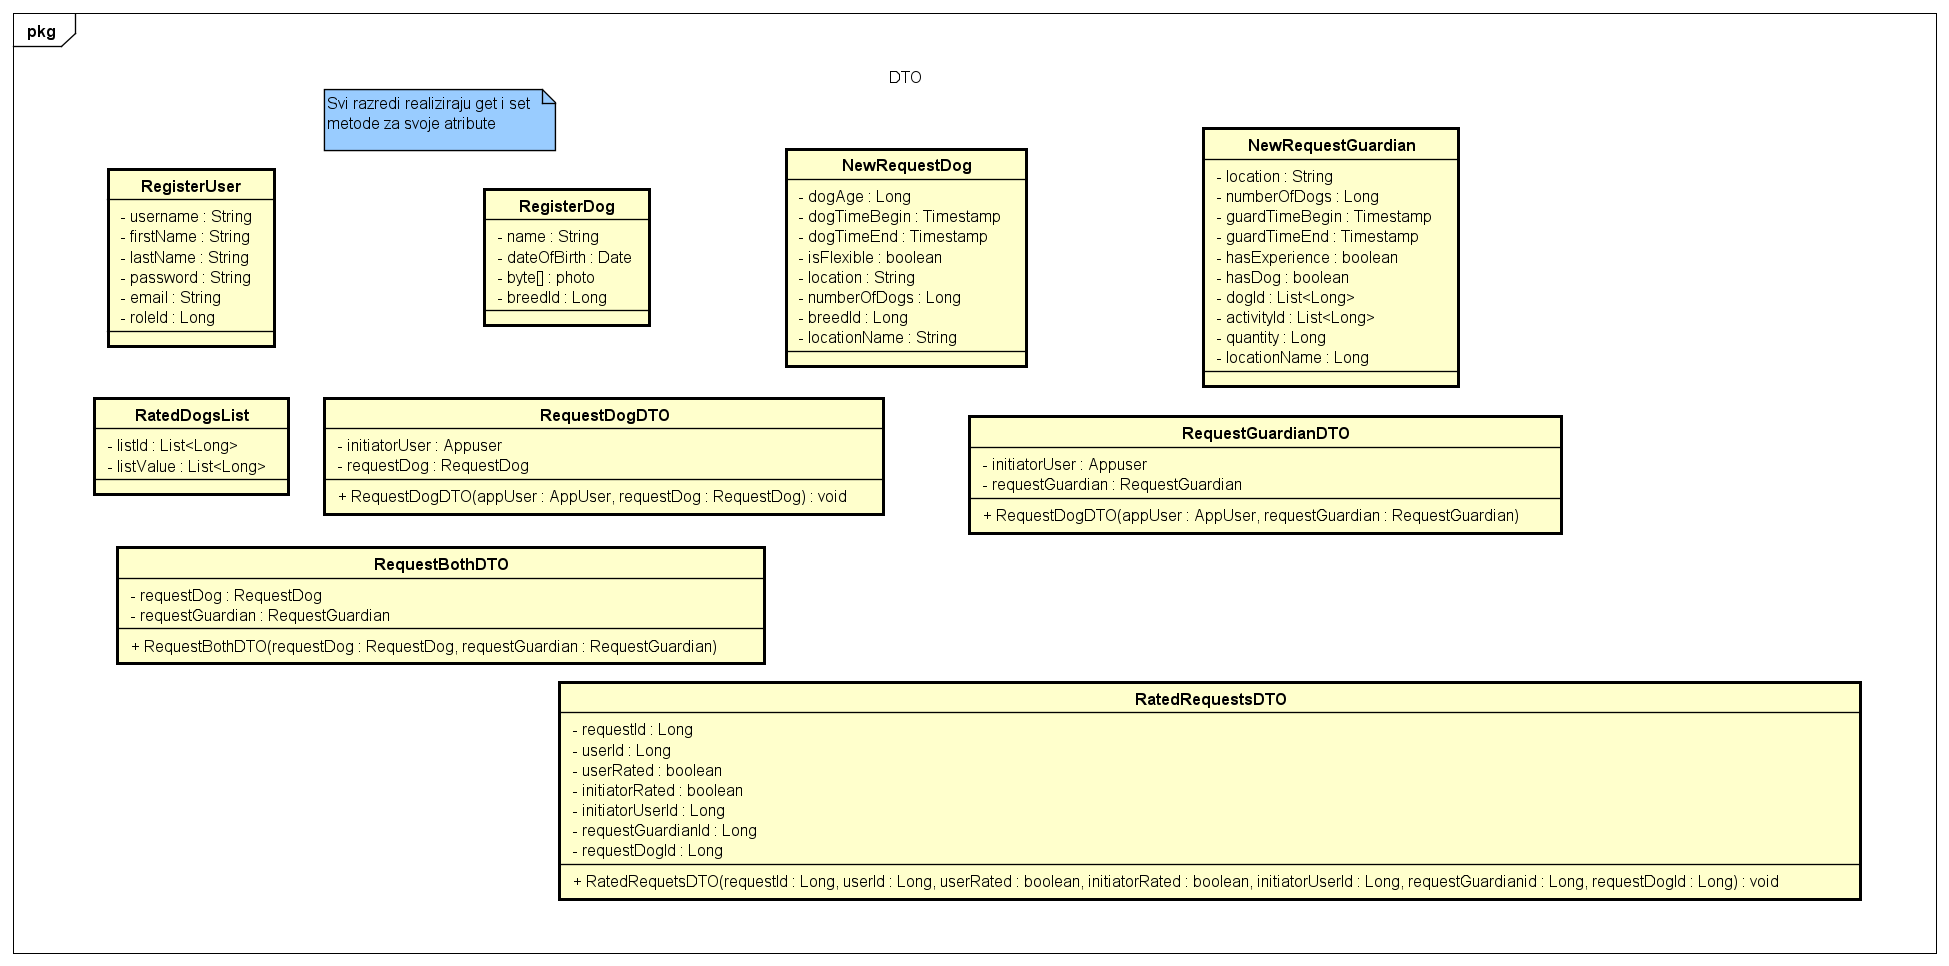
\includegraphics[width=15cm]{slike/Dijagram razreda - DTO}
				\caption{Dijagram razreda - dio Data Transfer Objects}
				\label{fig:Class-Diagram}
			\end{figure}
		
		
			Domain razredi preslikavaju strukturu baze podataka u aplikaciji. Implementirane metode direktno komuniciraju s bazom podataka te vraćaju tražene podatke.\\
			Razred AppUser predstavlja korisnika web aplikacije koji se može registrirati unos-eći potrebne informacije. On može izabrati svoju ulogu pri registraciji (razred Role). Administrator je korisnik aplikacije koji ima sve mogućnosti razreda AppUser. Vlasnik pasa može dodati vlastitog psa u sustav (razred Dog). Vlasnik, odnosno čuvar mogu tražiti čuvara za svog pasa (razred RequestGuardian), odnosno psa za čuvanje (razred RequestDog). Vlasnik može i tražiti koju aktivnost će čuvar raditi sa psom (razredi Activity i RequestActivity). Dogovor vlasnika i čuvara predstavlja razred AgreedRequest. U RequestGuardiansDog se popisuju psi koju se koriste u zahtjevu RequestGuardian.
			
			\begin{figure}[htb]
				\centering
				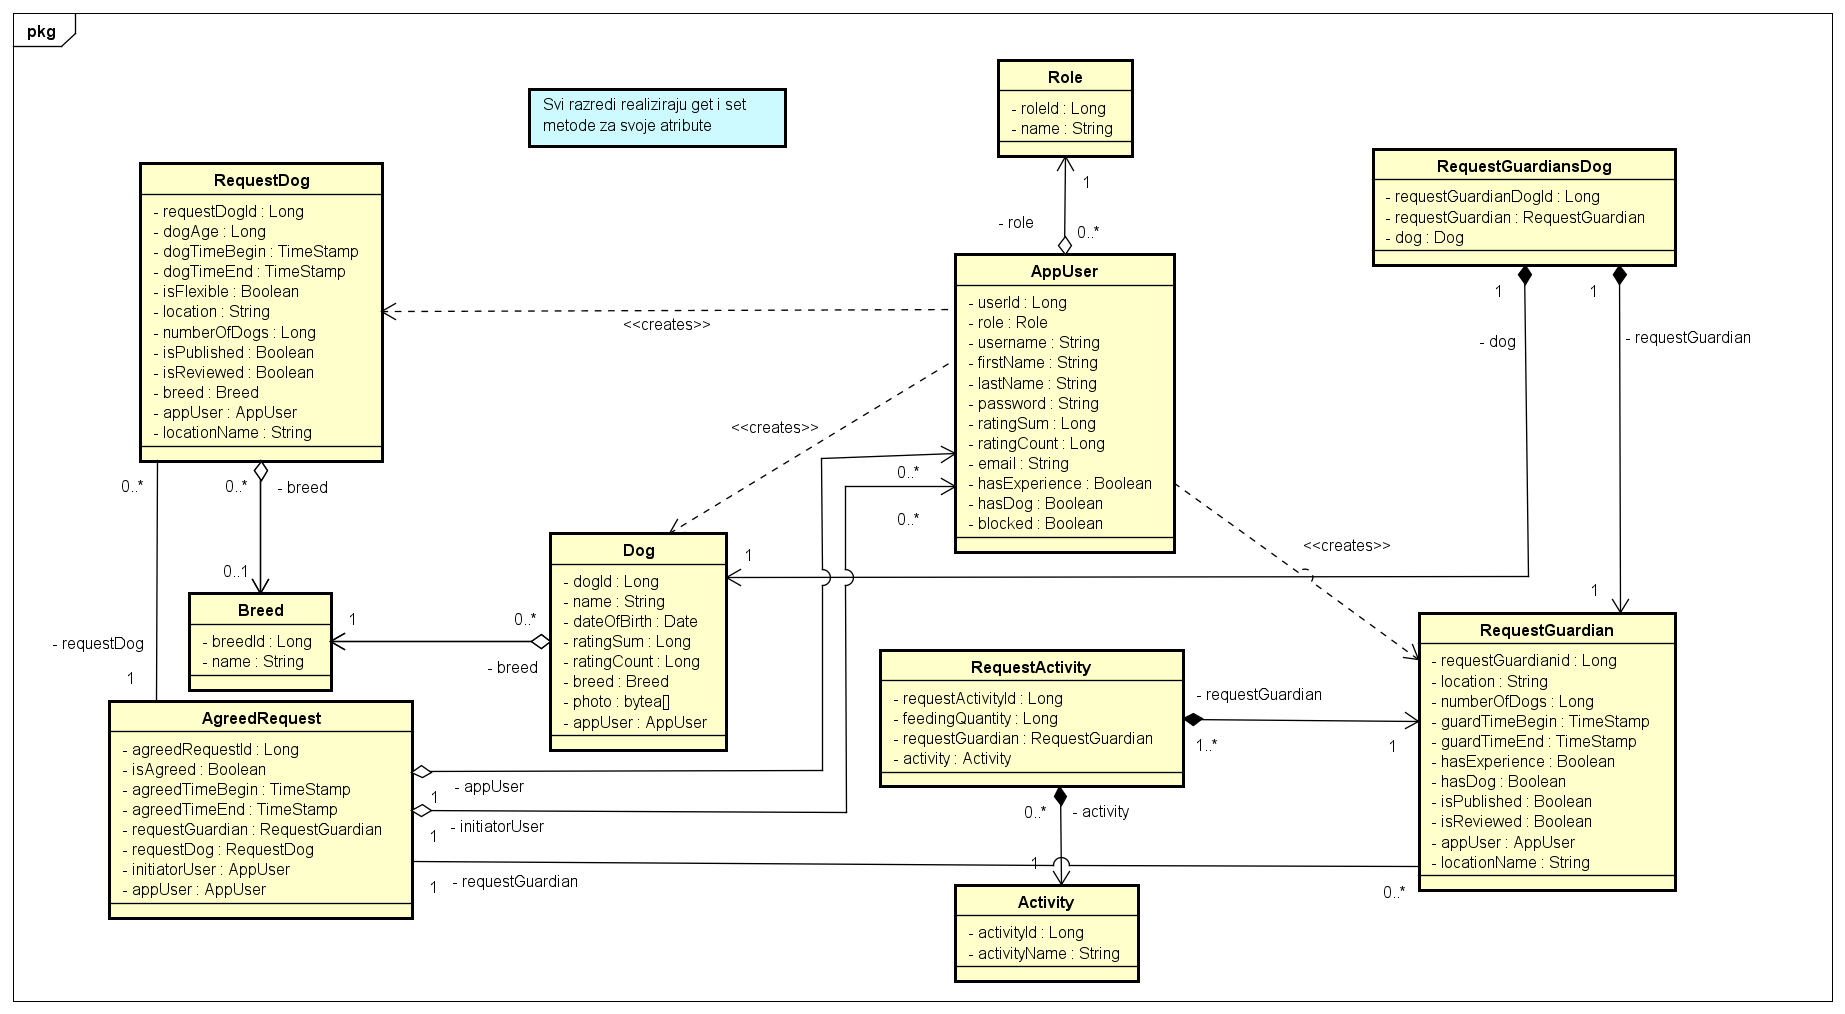
\includegraphics[width=15cm]{slike/Dijagram razreda - Domain}
				\caption{Dijagram razreda - dio Domain}
				\label{fig:Class-Diagram}
			\end{figure}
	
			\eject
		
		\section{Dijagram stanja}
			
			
			%\textbf{\textit{dio 2. revizije}}\\
			
			%\textit{Potrebno je priložiti dijagram stanja i opisati ga. Dovoljan je jedan dijagram stanja koji prikazuje \textbf{značajan dio funkcionalnosti} sustava. Na primjer, stanja korisničkog sučelja i tijek korištenja neke ključne funkcionalnosti jesu značajan dio sustava, a registracija i prijava nisu. }
			
			Dijagram stanja prikazuje stanja objekta te prijelaze među stanjima koji su potaknuti okidačima. Na slici 4.6 prikazan je dijagram stanja prijavljenog korisnika s ulogom administratora. Nakon prijave u sustav korisnik se nalazi na početnoj stranici na kojoj može pročitati više informacija o samom sustavu. Kroz zaglavlje aplikacije može pristupiti svim objavljenim zahtjevima i oglasima, a kroz padajući izbornik u zaglavlju može pristupiti svom računu, stranici za upravljanje korisnicima te zahtjevima i oglasima, vlastitim zahtjevima i oglasima, vlastitim psima, pristiglim ponudama te se može odjaviti iz sustava. Pošto se zaglavlje nalazi na svim stranicama aplikacije, korisnik prethodno navedenim opcijama ima pristup gdje god da se nalazi u aplikaciji. Na stranici sa svim objavljenim zahtjevima ima mogućnost dodavanja novog zahtjeva te mogućnost javljanja na pojedine zahtjeve, a na stranici sa svim objavljenim oglasima ima mogućnost dodavanja novog oglasa te mogućnost javljanja na pojedine oglase. Na stranici s vlastitim zahtjevima ima mogućnost odabira najbolje ponude oglasa za pojedini zahtjev koju potom može prihvatiti ili odbiti, a isto može i na stranici s vlastitim oglasima. Stranici za pregled vlastitih pasa korisnik može pristupiti kroz padajući izbornik, ali i kroz pregled vlastitog računa te potom tamo ima mogućnost dodavanja novog psa.
			
			
			\begin{figure}[htb]
				\centering
				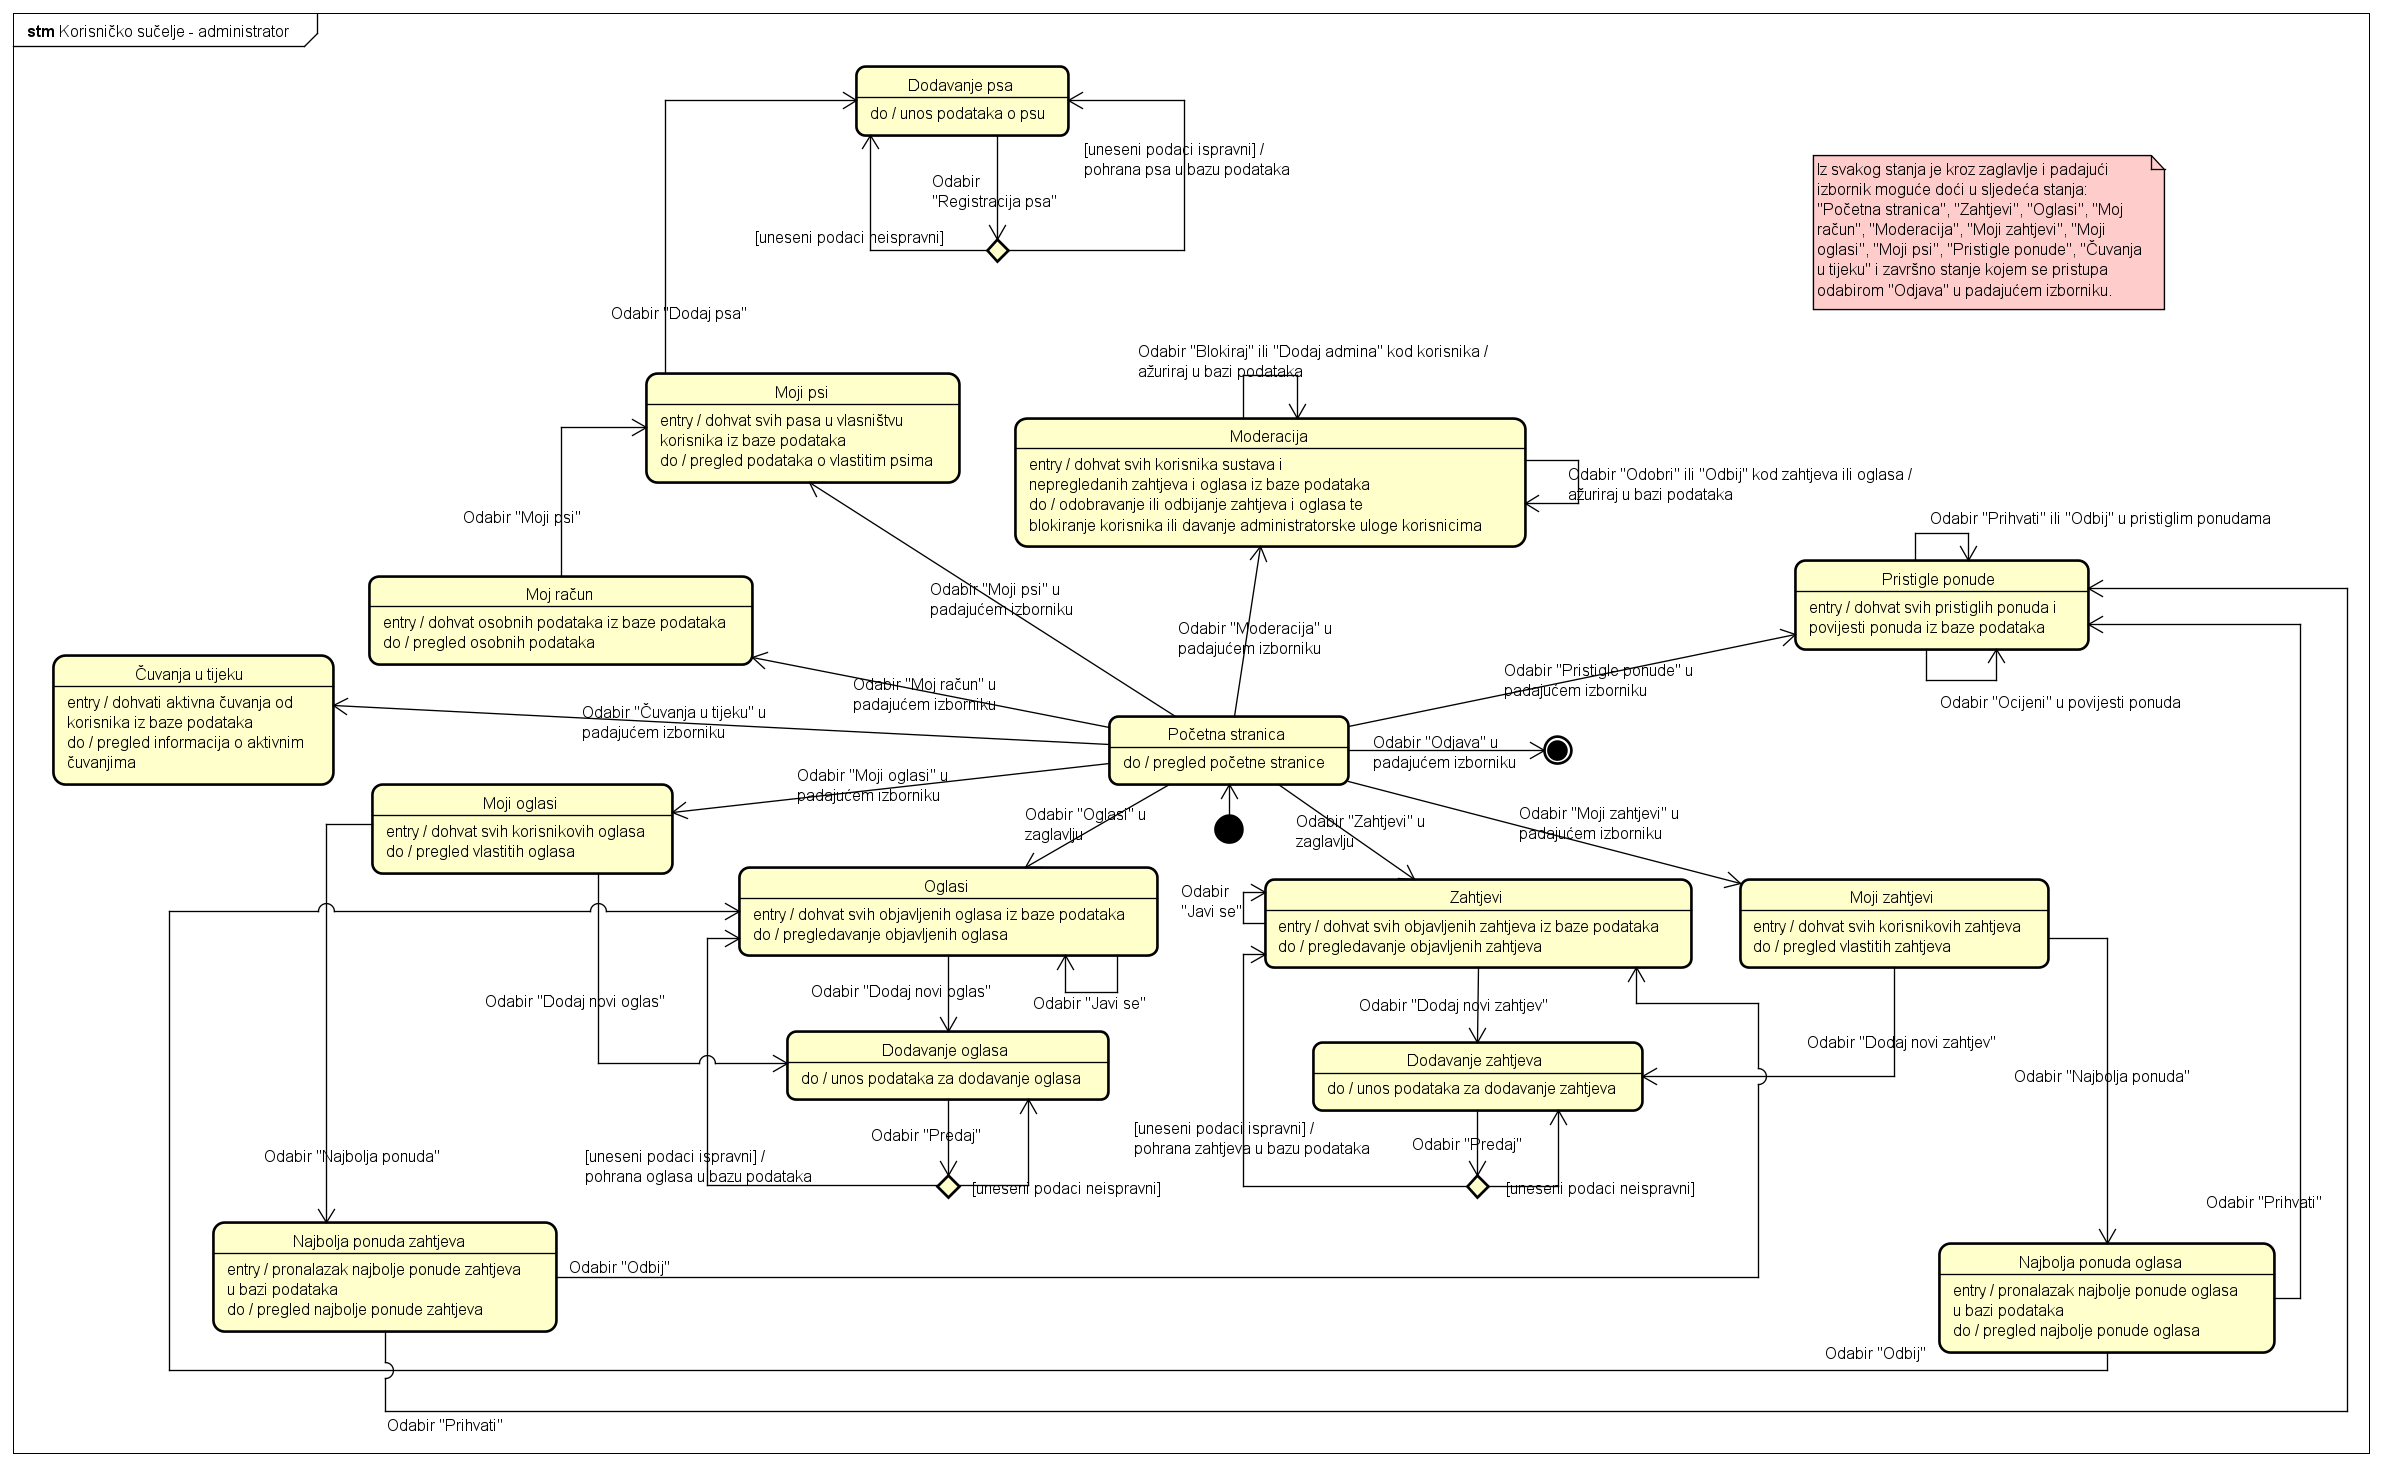
\includegraphics[width=15cm]{slike/Dijagram stanja}
				\caption{Dijagram stanja}
				\label{fig:State-Diagram}
			\end{figure}
			
			\eject 
		
		\section{Dijagram aktivnosti}
			
			Dijagram aktivnosti primjenjuje se za opis modela toka upravljanja ili toka podataka. Ne upotrebljava se za modeliranje događajima poticanog ponašanja. U
			modeliranju toka upravljanja svaki novi korak poduzima se nakon završenog prethodnog, a naglasak je na jednostavnosti. Na dijagramu aktivnosti sa slike 4.7 prikazan je proces sinkronizacije vlasnika i čuvara, odobravanje upita te ocjenjivanje. Vlasnik, čuvar i administrator se prijave u sustav. Vlasnik dodaje svog psa te radi zahtjev dok čuvar radi svoj oglas.
			Ako je sve u redu administrator potvrđuje te upite i započinje sinkronizacija između vlasnika i čuvara. Nakon što je čuvanje završilo, vlasnik može ocijeniti čuvara dok čuvar može ocijeniti pse.
			
			
			
			\begin{figure}[H]
				\centering
				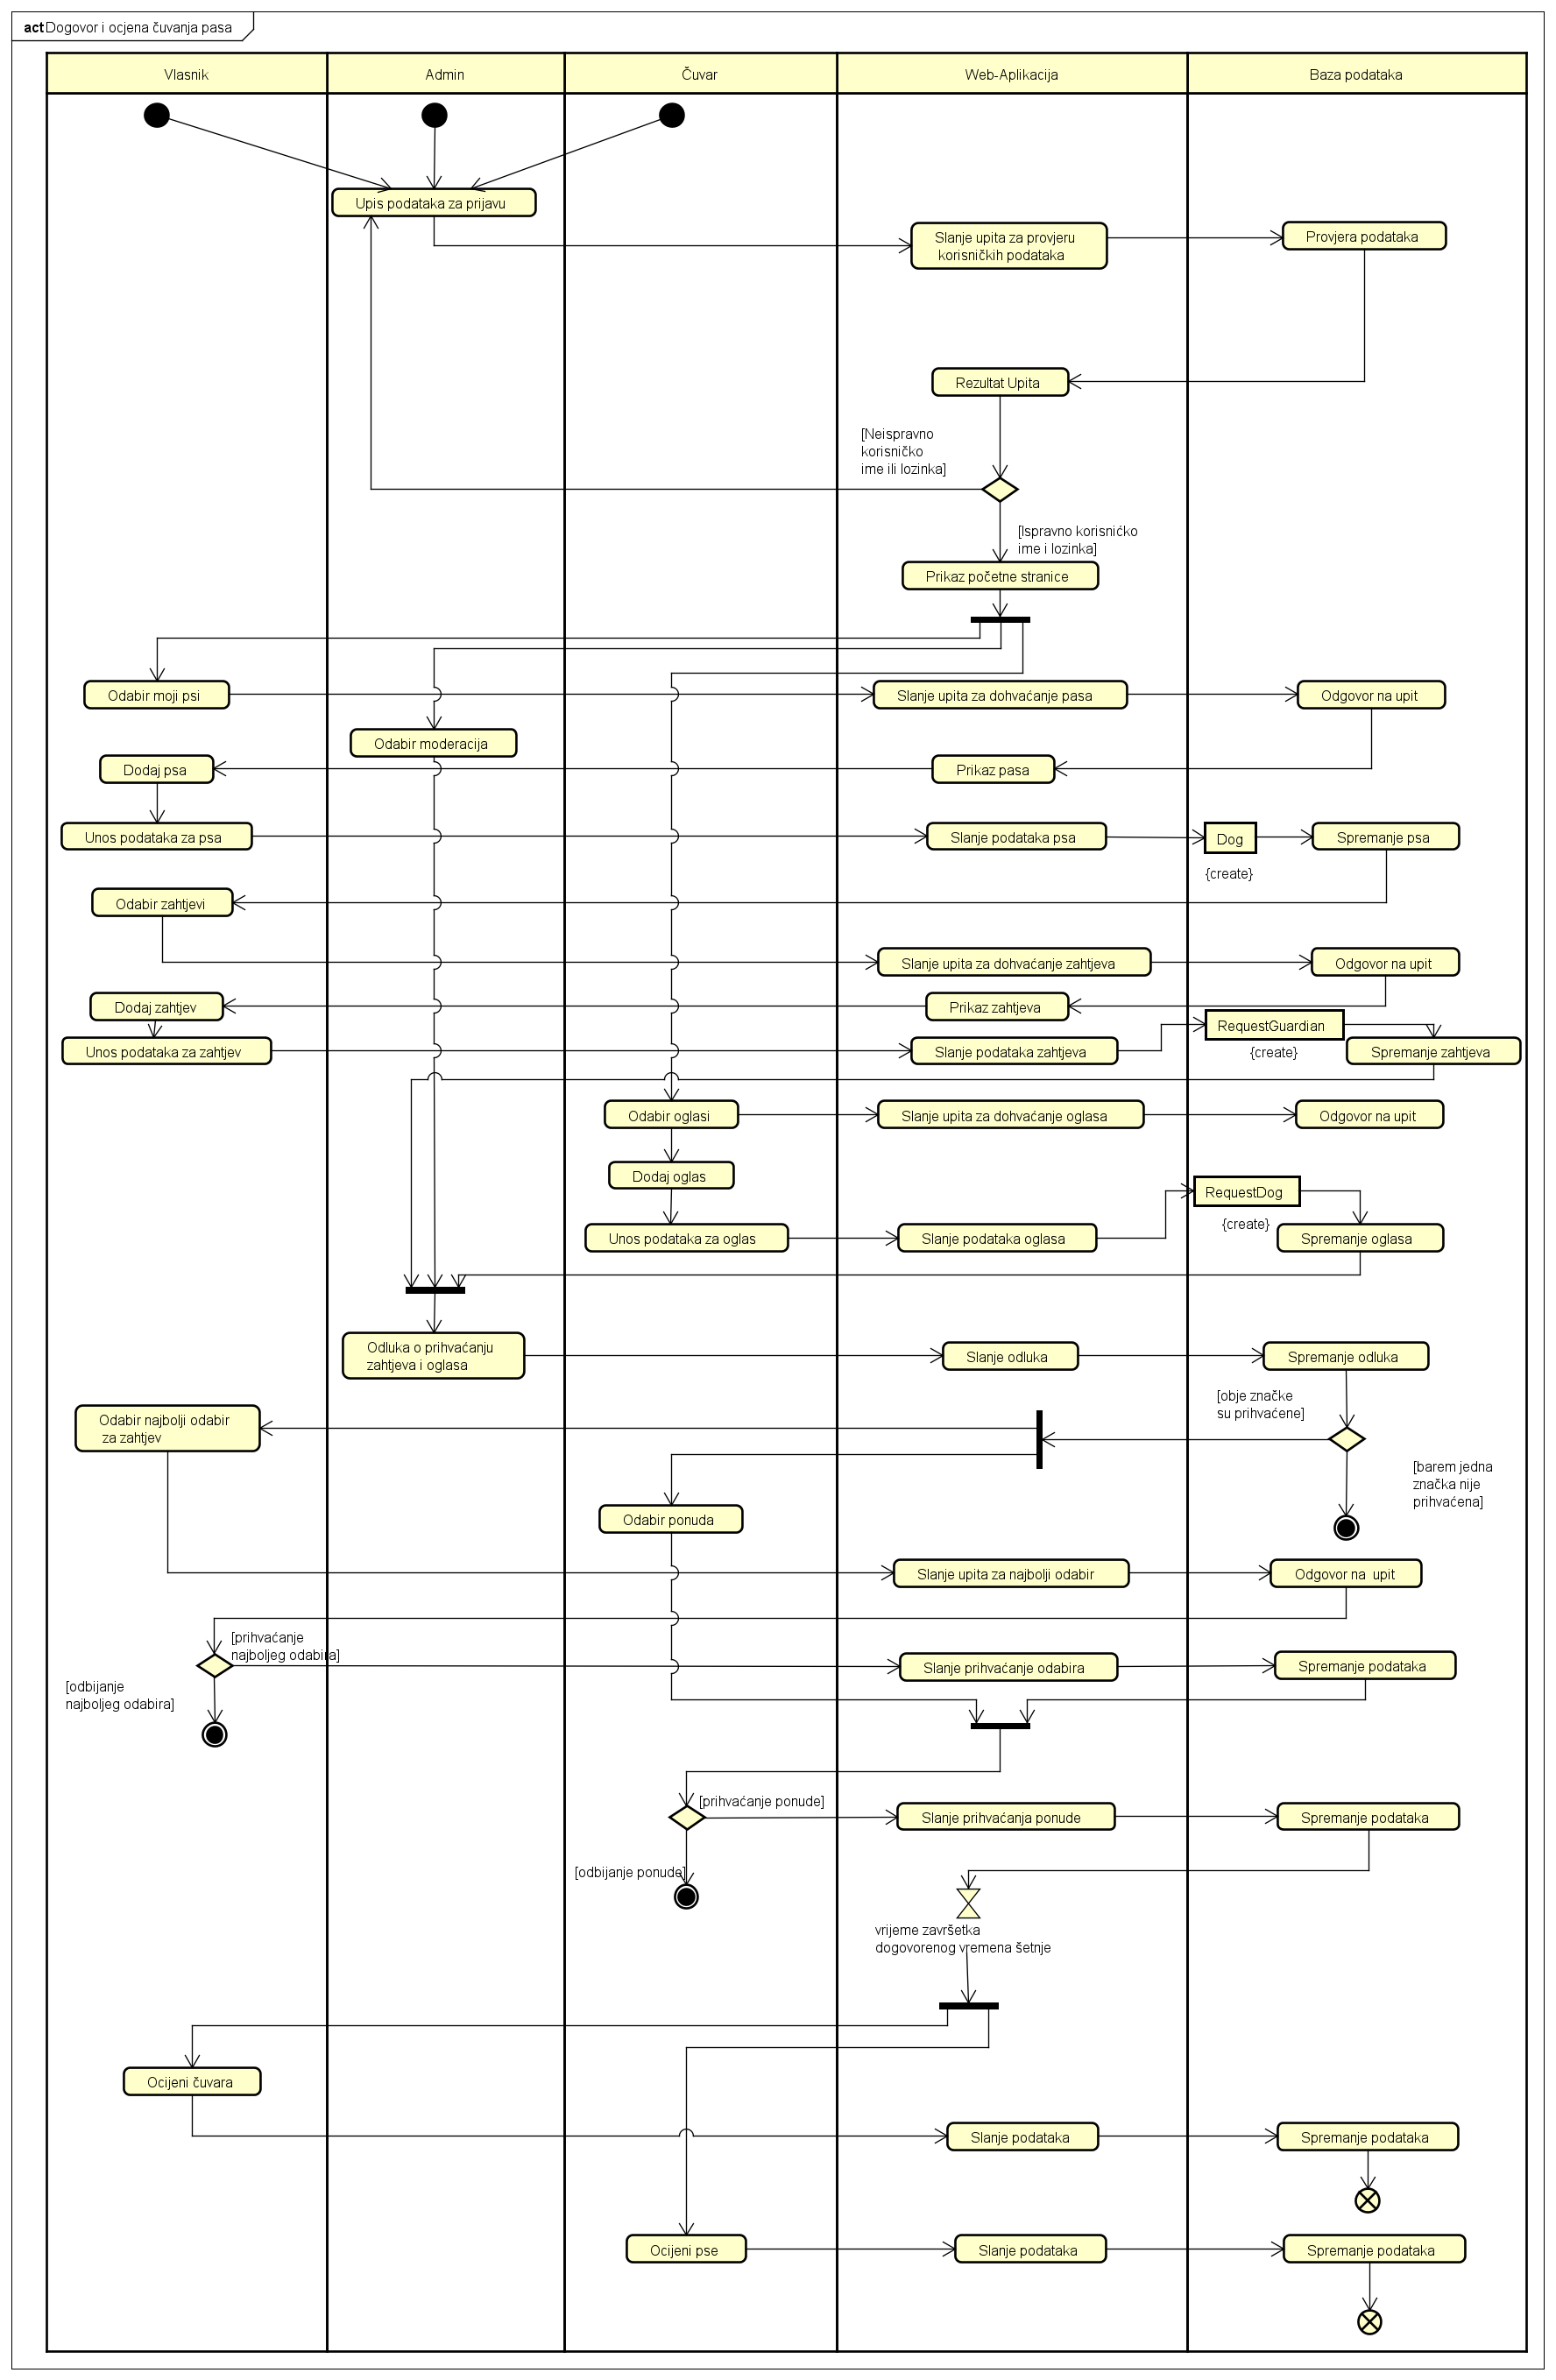
\includegraphics[width=15cm]{slike/Dijagram aktivnosti}
				\caption{Dijagram aktivnosti}
				\label{fig:Activity-Diagram}
			\end{figure}
			
			 
			
			\eject
		\section{Dijagram komponenti}
		
			%\textbf{\textit{dio 2. revizije}}\\
		
			 %\textit{Potrebno je priložiti dijagram komponenti s pripadajućim opisom. Dijagram komponenti treba prikazivati strukturu cijele aplikacije.}
			 Dijagram komponenti je strukturni dijagram kojim se vizualizira organizacija i međuovisnost između implementacijskih komponenti te odnos programske potpore prema okolini. Dijagram komponenti na slici 4.8 sastoji se od komponente web preglednika, baze podataka, te same aplikacije koja ima svoje dvije glavne podkomponente, a to su frontend i backend. U web pregledniku se preko sučelja za dohvat vizualnih datoteka prikazuju pojedine stranice. O tome koja će se datoteka dohvatiti, odnosno stranica prikazati odlučuje React router komponenta frontenda na temelju URL-a kojem se pristupa. Frontend se još sastoji od komponenti React view, index.js i ReactJS koje su međusobno zavisne. ReactJS je sama biblioteka iz koje se dobivaju gotove komponente za prikaz. index.js služi kao početna komponenta unutar koje se nalazi organizirana hijerarhija ostalih elemenata za prikaz. Rect view komponenta pak komunicira s backendom preko REST API-ja i razmjenjuje podatke s backendom u JSON formatu, a ovisno o korisnikovim akcijama osvježava prikaz na stranici. Controller komponenta backenda prima zahtjeve, preovjerava ih te šalje odgovore na dobivene zahtjeve prema klijentskoj strani. Backend se još sastoji od komponente Service koja prima zahtjeve od Controllera, obrađuje ih i prosljeđuje komponenti Repository koja onda preko JPA sučelja komunicira sa PostgreSQL bazom podataka u koju se pohranjuju podaci.
			 
			 \begin{figure}[H]
			 	\centering
			 	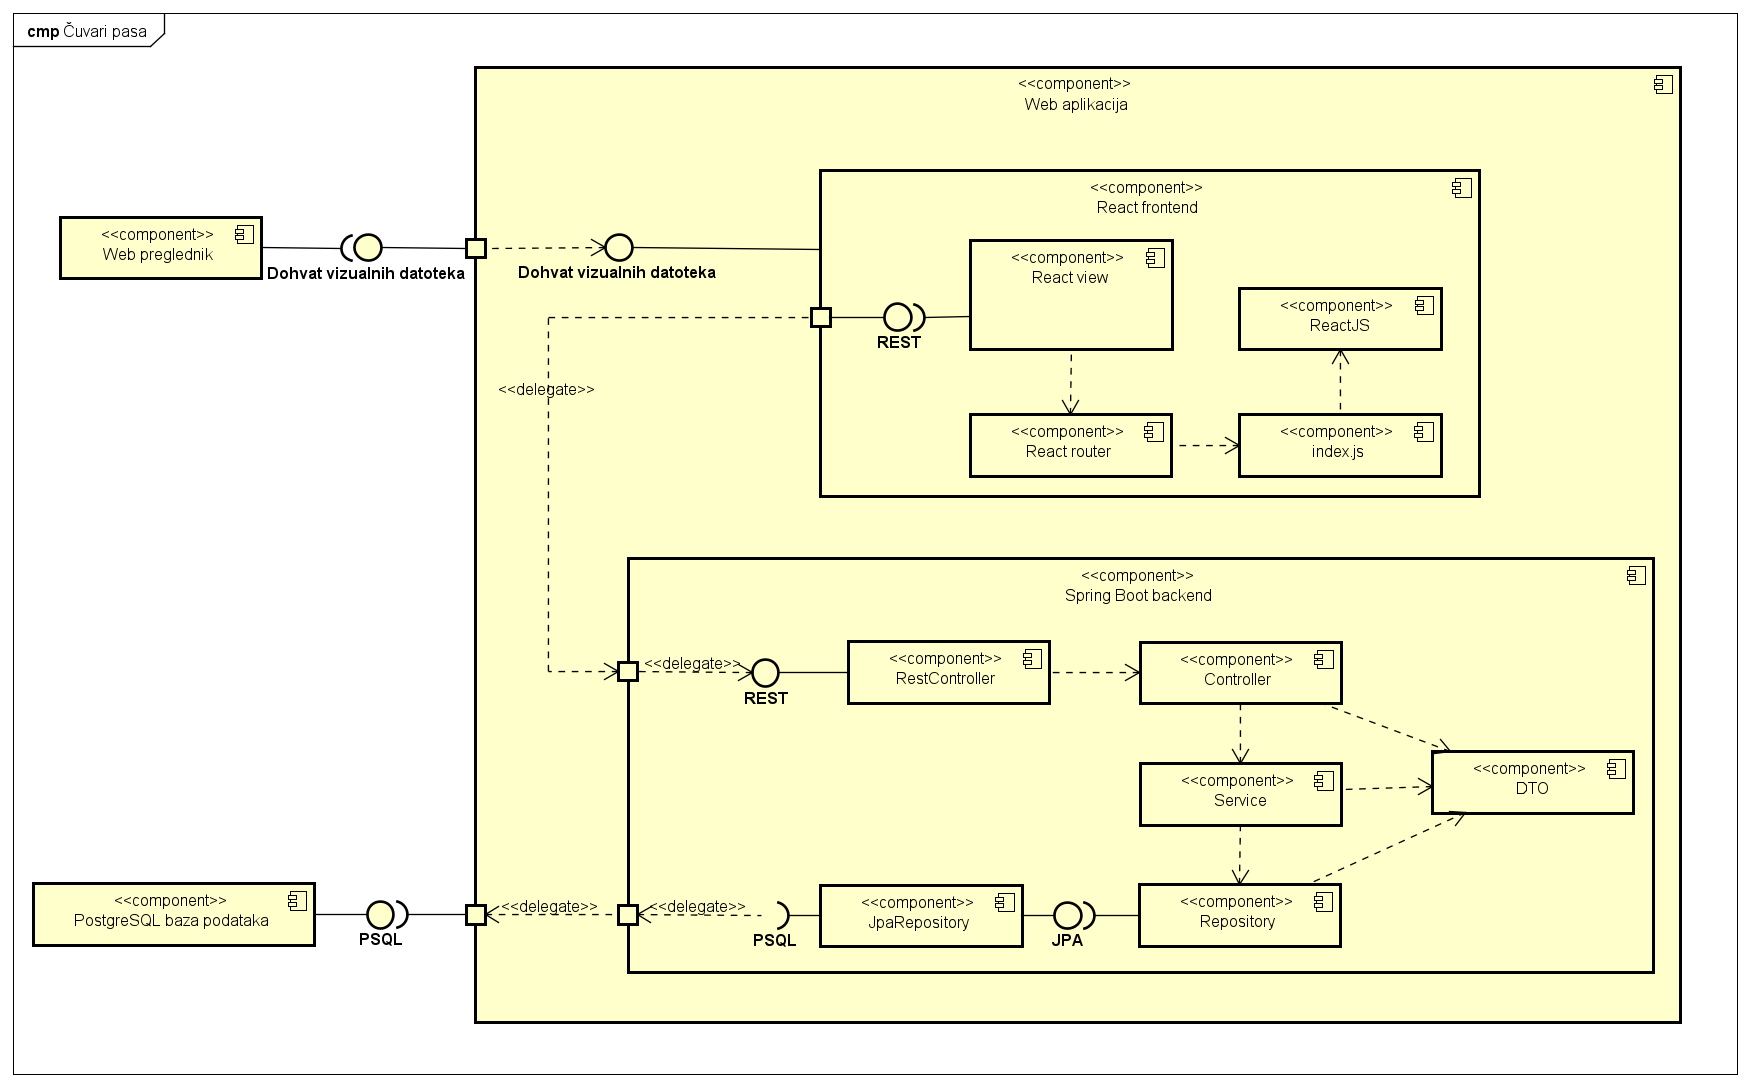
\includegraphics[width=15cm]{slike/Dijagram komponenti}
			 	\caption{Dijagram komponenti}
			 	\label{fig:Component-Diagram}
			 \end{figure}